\subsection{Francesco Foschini}
Il mio compito all'interno del progetto, è stato quello di modellare la gerarchia di \texttt{Entity} del gioco.
In particolare mi sono occupato della implementazione del model degli zombie, dei proiettili e l'attore che definisce il comportamento dei proiettili.
Ho partecipato inoltre allo sviluppo del \texttt{Troop Actor} del \texttt{Menù Screen} e del \texttt{Game Screen}.

\subsubsection{Bullet}
I proiettili rappresentano all'interno del gioco l'attacco delle \texttt{Plant} e degli \texttt{Zombie}.\\

Grazie alla buona gerarchia di caratteristiche definite in \texttt{Entity}, è stato possibile grazie  ai \textbf{mixins},
dotare il trait \texttt{Bullet} dell'abilità di movimento \texttt{Movement Ability}.
Il trait \texttt{Bullet} rappresenta quindi l'entità base "sparata" da una \texttt{Troop}.
Tutti i \texttt{Bullet} presentano un comportamento comune: hanno una posizione, una velocità, una dimensione ed un danno.\\


Successivamente sono stati individuati due diversi sottotipi\\ \texttt{Bullet}: \texttt{ZombieBullet} e \texttt{PlantBullet}.
Il primo è il trait che modella il colpo base degli \texttt{Zombie} mentre il secondo si riferisce all'attacco base delle \texttt{Plant}.

Attraverso il metodo \texttt{checkCollision} i \texttt{PlantBullet} possono collidere solamente contro le entità di tipo \texttt{Zombie} mentre,
al contrario, gli \texttt{ZombieBullet} potranno colpire solamente le entità sottotipo di \texttt{Plant}.

Mi sono successivamente concentrato nell'implementazione di due tipi di \texttt{ZombieBullet}: \texttt{PawBullet} (il bullet dei
\texttt{BasicZombie} e \texttt{FastZombie}) e lo \\
\texttt{SwordBullet} (il bullet dei \texttt{WarriorZombie}).
Lo \texttt{SwordBullet} è un attacco più potente rispetto al \texttt{PawBullet}.\\

Volendo seguire un approccio puramente funzionale, favorendo l'immutabilità delle entità, il metodo di
aggiornamento della posizione di un \texttt{Bullet} deve crearne uno nuovo con la posizione aggiornata.
Questo comportamento è comune a tutti i tipi di \texttt{Bullet}. L'aggiornamento deve, inoltre,
tornare il tipo di \texttt{Bullet} corretto. A tal proposito è stato utilizzato il metodo di scala  \textbf{copy()} che può essere utilizzato solo nelle \texttt{case class}. Tutte le classi che estendono
\texttt{Bullet}, quindi, lo utilizzano per restituire un nuovo \texttt{Bullet} con la posizione aggiornata.
Attraverso questa strategia si può utilizzare la \textbf{infix notation} per aggiornare la posizione dei \texttt{Bullet}.

\begin{lstlisting}[language=Scala, label=code:bullet-update, caption=aggiornamento di un bullet. ]
    bullet withPosition Position(1, 0)
\end{lstlisting}



La stessa soluzione è stata poi adottata anche nelle \texttt{Troop}.

La velocità e il danno di ogni tipo di bullet sono definiti dentro l'oggetto \texttt{BulletDefaultValues}.

Per istanziare ogni tipo di \texttt{Bullet} abbiamo pensato di utilizzare il \textbf{pattern builder}.
Dentro all'object \texttt{Bullets} è stato creato un \texttt{trait BulletBuilder}
con un unico metodo \textit{build} che ritorna uno specifico tipo di \texttt{Bullet}.
Utilizzando le \textbf{given conversion} sono state definite tante \texttt{BulletBuilder} per ogni sottotipo di \texttt{Bullet} da istanziare.
E' stato, infine, definito un metodo \textit{ofType} che, dato un tipo
di \texttt{Bullet}, chiama il builder corretto per restituire la nuova entità.

\begin{lstlisting}[language=Scala, label=code:troop-builder, caption= Builder per la creazione di una Troop.]
object Bullets:
      /**
       * A builder used to create [[Bullet]].
       *
       * @tparam T The type of the [[Bullet]].
       */
      trait BulletBuilder[B <: Bullet]:
        /**
         * @return A [[Bullet]] of type [[B]]
         */
        def build: B

      /**
       * Given instances to create a [[PeaBullet]].
       */
      given BulletBuilder[PeaBullet] with
        override def build: PeaBullet = PeaBullet()

      /**
       * Given instances to create a [[SnowBullet]].
       */
      given BulletBuilder[SnowBullet] with
        override def build: SnowBullet = SnowBullet()

      /**
       * Given instances to create a [[CherryBullet]].
       */
      given BulletBuilder[CherryBullet] with
        override def build: CherryBullet = CherryBullet()

      /**
       * Given instances to create a [[PawBullet]].
       */
      given BulletBuilder[PawBullet] with
        override def build: PawBullet = PawBullet()

      /**
       * Given instances to create a [[SwordBullet]].
       */
      given BulletBuilder[SwordBullet] with
        override def build: SwordBullet = SwordBullet()

      /**
       * A DSL method to create every type of [[Bullet]].
       *
       * @param bulletBuilder The [[BulletBuilder]] of the type needed.
       * @tparam B The [[Bullet]] type.
       * @return The [[Bullet]] of the specified type.
       */
      def ofType[B <: Bullet](using bulletBuilder: BulletBuilder[B]): B =
        bulletBuilder.build
\end{lstlisting}

Viene mostrato di seguito come istanziare un PawBullet:

\begin{lstlisting}[language=Scala, label=bullet-creation, caption=Bullet creation. ]
    val bullet = Bullets.ofType[PawBullet]
\end{lstlisting}

\begin{figure}[H]
    \centering
    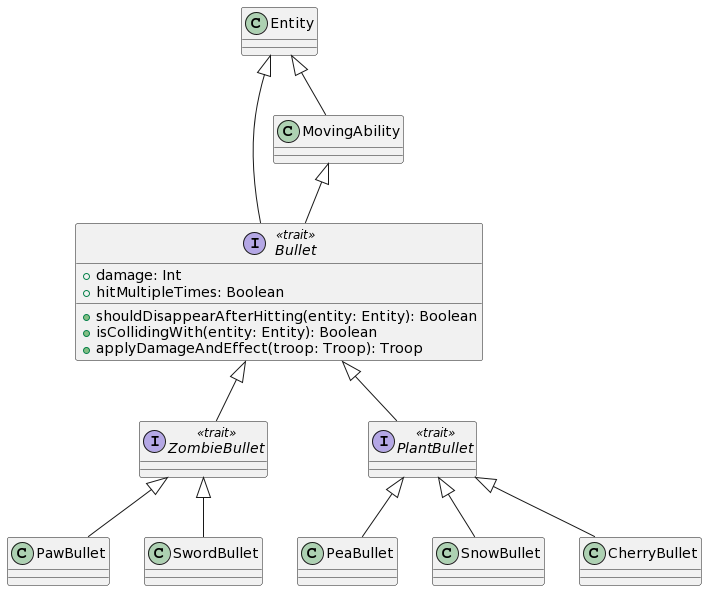
\includegraphics[width=1\linewidth]{images/model-bullet}
    \caption{Diagramma delle classi rappresentante i \texttt{ZombieBullet}.}
    \label{fig:class-bullet}
\end{figure}

Il model del \texttt{Bullet} è stato testato nella classe \texttt{BulletModelTest}.

\subsubsection{BulletActor}
Avendo adottando un'architettura ad attori, abbiamo pensato di incapsulare il comportamento
di ogni proiettile dentro un \texttt{BulletActor}. Quindi, in fase di creazione, ogni \texttt{Bullet} sarà associato ad un
\texttt{BulletActor} che ne definirà il comportamento.
Il \texttt{BulletActor} ha un solo Behaviour chiamato \texttt{moving}: risponde ai messaggi ricevuti dal \texttt{GameLoop}.

Come il \texttt{TroopActor}, ad ogni iterazione del \texttt{GameLoop} il \texttt{BulletActor} riceve un messaggio di \texttt{Update()} a seguito del quale:
\begin{enumerate}
    \item Aggiorna il proprio \texttt{Bullet}.
    \item Manda il suo \texttt{Bullet} aggiornato al \texttt{GameLoop}.
    \item Ricrea il proprio Behaviour con il \texttt{Bullet} aggiornato.
\end{enumerate}
Quando il \texttt{Bullet} collide con un'altra entità riceve un messaggio \texttt{Collision()} a seguito del quale:
\begin{enumerate}
    \item Crea il \texttt{Bullet} della propria \texttt{Troop}.
    \item Crea un \texttt{BulletActor} che controlla il \texttt{Bullet}.
    \item Notifica il \texttt{GameLoop} dell'avvenuta creazione con il messaggio \texttt{BulletSpawned()}.
\end{enumerate}
\newpage
Il comportamento del \texttt{BulletActor} viene mostrato nel seguente diagramma:
\begin{figure}[H]
    \centering
    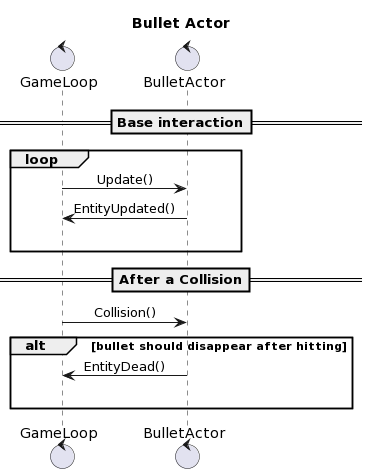
\includegraphics[width=0.8\linewidth]{images/bullet-actor.png}
    \caption{Diagramma di sequenza del Bullet Actor.}
\end{figure}

Il \texttt{BulletActor} è stato testato nella classe \texttt{BulletActorTest} utilizzando il framework \textbf{AkkaTest}.

\subsubsection{Zombie}
Gli \texttt{Zombie} rappresentano una delle entità fondamentali del gioco. In particolare, rappresentano i nemici che l'utente
deve cercare di eliminare attraverso il piazzamento delle piante nel campo di gioco.
Tutti gli \texttt{Zombie} sono in grado di muoversi orrizzontalmente nelle lane del campo di gioco con una certa velocità: pertanto
attraverso il meccanismo dei mixins il \texttt{trait Zombie} estende il \texttt{trait Troop} a cui aggiunge poi l' abilità \texttt{MovingAbility}.

Quando uno \texttt{Zombie} è colpito da un \texttt{SnowBullet} potrebbe essere rallentato, per questo motivo si è deciso di
mettere la velocità in ciascun costruttore per ciascun tipo di \texttt{Zombie} implementato.
In questo modo, seguendo un approccio funzionale e favorendo l'immutabilità delle istanze, quando lo \texttt{SnowBullet} collide con uno specifico \texttt{Zombie}
istanzierà nuovamente lo \texttt{Zombie} con la velocità aggiornata.
A tal proposito è stata implementata una val \texttt{slowVelocities} dentro all'object \texttt{ZombieDefaultValues}.

E' infatti nell'object \texttt{ZombieDefaultValue} che sono definite tutte le caratteristiche principali per ogni
tipo di \texttt{Zombie} implementato: stato iniziale e di default (\texttt{Moving}), vita iniziale,
il tipo \texttt{Bullet} a disposizione, la velocità di default, la velocità degli \texttt{Zombie} rallentati e un metodo per generare
la posizione iniziale degli \texttt{Zombie}.

Come mostrato nel diagramma delle classi degli \texttt{Zombie}, ogni classe che rappresenta uno \texttt{Zombie} deve estendere dal \texttt{trait Zombie}.

\begin{figure}[H]
    \centering
    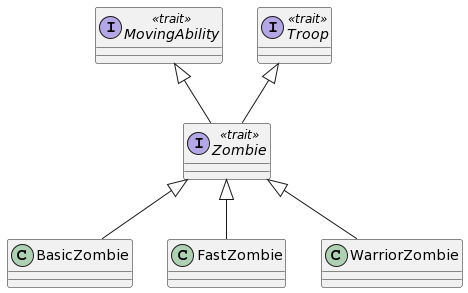
\includegraphics[width=1\linewidth]{images/model-zombie.png}
    \caption{Diagramma delle classi rappresentante gli \texttt{Zombie}.}
    \label{fig:class-zombie}
\end{figure}

Il comportamento degli \texttt{Zombie} è incapsulato nel \texttt{TroopActor} e il model degli \texttt{Zombie} è stato testato nella classe \texttt{ZombieModelTest}.
